\chapter{Results}

\label{chapter:results}

In this chapter, we focus on summarizing the results of our aforementioned
methodologies. As a note, we do not dive deep into answering our research
questions here. Instead, we simply use this chapter to report on our results and
we answer our research questions in the next chapter.

\section{RQ1: Evaluating performance of SoPa++}

Following our methodologies, we conducted a grid-search training paradigm where
we varied our patterns and $\tau$-threshold parameters to obtain a total of 15
different modelling runs. Given that we repeated unique model run 10 times, we
ultimately ran our grid-search for 150 model runs. This process took roughly 24
hours on a single NVIDIA GeForce GTX 1080 Ti GPU running light, medium and heavy
model runs concurrently.

\subsection{Training}

We first describe the results of our training. Figure \ref{fig:results_training}
shows the progress of the validation accuracy against training updates. The
different coloured lines indicate the various initial random seeds assigned to
the particulat model run. We can observe that increasing the $\tau$ value from 0
to 1 tends to decrease the overall validation accuracy profile. Correspondingly,
we can also observe that the larger model tends to have a higher validation
accuracy profile compared to the smaller models. We refer to the pattern
hyperparameter as $P$ in Figure \ref{fig:results_training}. Finally, we can
observe that the larger models tend to have an earlier convergence or
early-stopping window compared to the smaller models.

\subsection{Evaluation}

In regards to the evaluation of SoPa++ performance, we can refer to Table
\ref{tab:results_evaluation} for a tabular summary of test accuracies across the
light, medium and heavy model variants grouped by the various $\tau$-thresholds.
The exact specification of the light, medium and heavy model variants were
described in Section \ref{section:spp_training}. Here, we can observe that the
best performing models were the heavy models with $\tau$=0.0 and $\tau$=0.25
and the medium model with $\tau$=0.0. We can observe that test accuracies
generally show a decreasing trend as we increase the $\tau$-threshold.
Correspondingly, we can observe a decreasing performance trend as we decrease
the size of the model from heavy to light models. We can also observe that the
standard deviations in performance are generally similar.

\begin{figure}[t!]
  \centering
  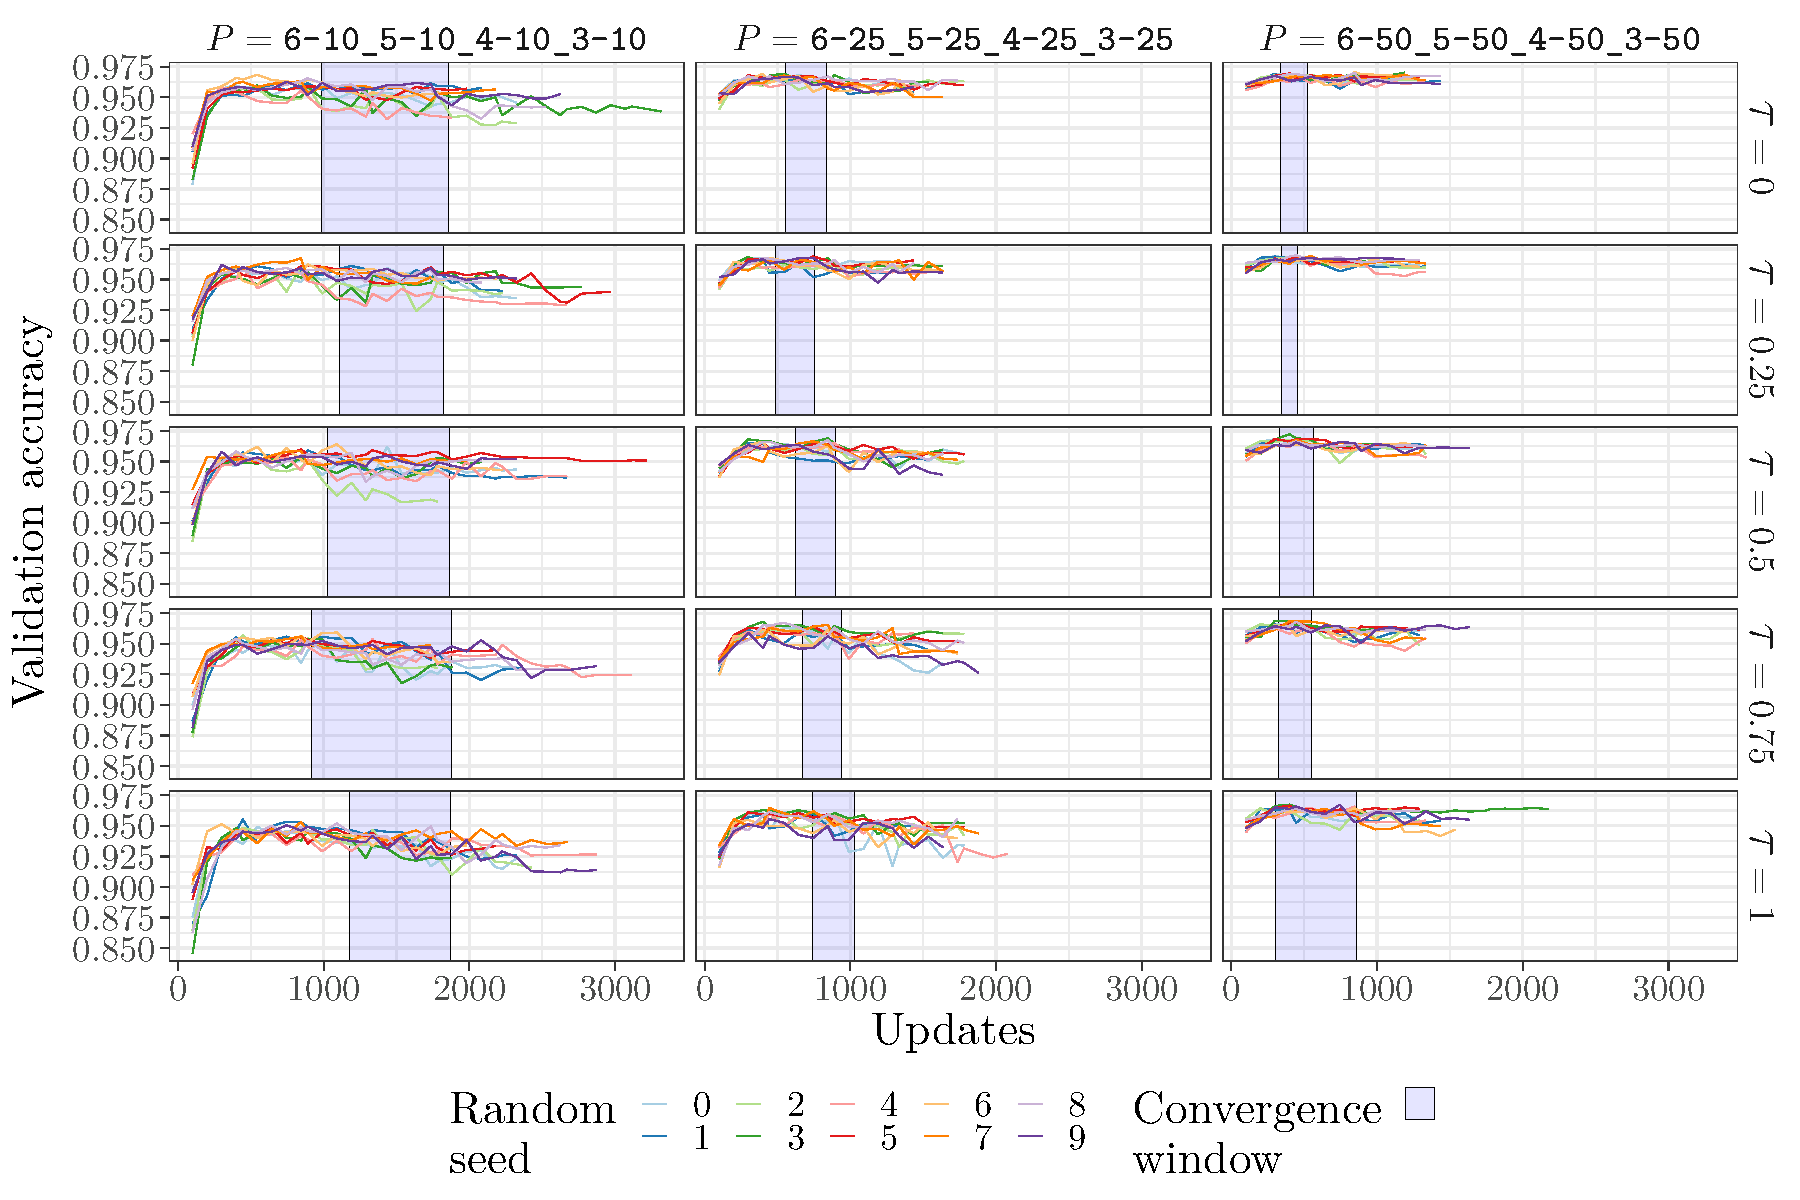
\includegraphics[width=14cm]{pdfs/generated/train_spp_grid_1617362157.pdf}
  \caption{Visualization of validation accuracy against number of training
    updates for grid-search grouped by pattern hyperparameters and $\tau$-thresholds}
  \label{fig:results_training}
\end{figure}

\begin{table}[t!]
  \centering \def\arraystretch{1.3}
  \small
  \begin{tabular}{lllllll}
    \toprule
    && \multicolumn{5}{c}{Accuarcy in $\%$ with mean $\pm$ standard-deviation} \\
    \cline{3-7} \\[-10pt]
    Model & Parameters & $\tau$=0.0 & $\tau$=0.25 & $\tau$=0.5 & $\tau$=0.75 & $\tau$=1.0 \\
    \midrule
    Light & 1,260,292 & 97.6 $\pm$ 0.2 & 97.6 $\pm$ 0.2 & 97.3 $\pm$ 0.2 & 97.0 $\pm$ 0.3 & 96.9 $\pm$ 0.3 \\
    Medium & 1,351,612 & \textbf{98.3 $\bm{\pm}$ 0.2} & 98.1 $\pm$ 0.1 & 98.0 $\pm$ 0.2 & 97.9 $\pm$ 0.1 & 97.7 $\pm$ 0.1  \\
    Heavy & 1,503,812 & \textbf{98.3 $\bm{\pm}$ 0.2} & \textbf{98.3 $\bm{\pm}$ 0.2} & 98.2 $\pm$ 0.2 & 98.1 $\pm$ 0.2 & 98.0 $\pm$ 0.2 \\
    \bottomrule
  \end{tabular}
  \caption{Test accuracies of the SoPa++ models grouped by model sizes and
    $\tau$-thresholds; accuracies and standard deviations were calculated across
  random seed iterations}
  \label{tab:results_evaluation}
\end{table}

\section{RQ2: Evaluating explanations by simplification}

% > aggregate(regex_acc ~ patterns + tau_threshold, data=collections, FUN=mean)
%               patterns tau_threshold regex_acc
% 1  6-10_5-10_4-10_3-10             0 0.9549596
% 2  6-25_5-25_4-25_3-25             0 0.9745687
% 3  6-50_5-50_4-50_3-50             0 0.9789218
% 4  6-10_5-10_4-10_3-10          0.25 0.9617385
% 5  6-25_5-25_4-25_3-25          0.25 0.9748113
% 6  6-50_5-50_4-50_3-50          0.25 0.9803639
% 7  6-10_5-10_4-10_3-10           0.5 0.9645957
% 8  6-25_5-25_4-25_3-25           0.5 0.9747305
% 9  6-50_5-50_4-50_3-50           0.5 0.9803369
% 10 6-10_5-10_4-10_3-10          0.75 0.9634906
% 11 6-25_5-25_4-25_3-25          0.75 0.9752022
% 12 6-50_5-50_4-50_3-50          0.75 0.9803100
% 13 6-10_5-10_4-10_3-10             1 0.9610243
% 14 6-25_5-25_4-25_3-25             1 0.9748518
% 15 6-50_5-50_4-50_3-50             1 0.9805256
% > aggregate(regex_acc ~ patterns + tau_threshold, data=collections, FUN=sd)
%               patterns tau_threshold   regex_acc
% 1  6-10_5-10_4-10_3-10             0 0.009687851
% 2  6-25_5-25_4-25_3-25             0 0.005038281
% 3  6-50_5-50_4-50_3-50             0 0.004365320
% 4  6-10_5-10_4-10_3-10          0.25 0.008446945
% 5  6-25_5-25_4-25_3-25          0.25 0.003450913
% 6  6-50_5-50_4-50_3-50          0.25 0.003337103
% 7  6-10_5-10_4-10_3-10           0.5 0.005537846
% 8  6-25_5-25_4-25_3-25           0.5 0.002384975
% 9  6-50_5-50_4-50_3-50           0.5 0.002853588
% 10 6-10_5-10_4-10_3-10          0.75 0.006689082
% 11 6-25_5-25_4-25_3-25          0.75 0.002635605
% 12 6-50_5-50_4-50_3-50          0.75 0.002482981
% 13 6-10_5-10_4-10_3-10             1 0.006328909
% 14 6-25_5-25_4-25_3-25             1 0.003111233
% 15 6-50_5-50_4-50_3-50             1 0.002347448

% > aggregate(softmax_distance ~ patterns + tau_threshold, data=collections, FUN=mean)
%               patterns tau_threshold softmax_distance
% 1  6-10_5-10_4-10_3-10             0       0.15010717
% 2  6-25_5-25_4-25_3-25             0       0.09476992
% 3  6-50_5-50_4-50_3-50             0       0.07106383
% 4  6-10_5-10_4-10_3-10          0.25       0.11310785
% 5  6-25_5-25_4-25_3-25          0.25       0.07315419
% 6  6-50_5-50_4-50_3-50          0.25       0.04993503
% 7  6-10_5-10_4-10_3-10           0.5       0.09955704
% 8  6-25_5-25_4-25_3-25           0.5       0.06148820
% 9  6-50_5-50_4-50_3-50           0.5       0.04293018
% 10 6-10_5-10_4-10_3-10          0.75       0.10031126
% 11 6-25_5-25_4-25_3-25          0.75       0.05843249
% 12 6-50_5-50_4-50_3-50          0.75       0.04462260
% 13 6-10_5-10_4-10_3-10             1       0.10272472
% 14 6-25_5-25_4-25_3-25             1       0.06345463
% 15 6-50_5-50_4-50_3-50             1       0.04730200
% > aggregate(softmax_distance ~ patterns + tau_threshold, data=collections, FUN=sd)
%               patterns tau_threshold softmax_distance
% 1  6-10_5-10_4-10_3-10             0      0.022698184
% 2  6-25_5-25_4-25_3-25             0      0.016573534
% 3  6-50_5-50_4-50_3-50             0      0.014613714
% 4  6-10_5-10_4-10_3-10          0.25      0.021730004
% 5  6-25_5-25_4-25_3-25          0.25      0.009497534
% 6  6-50_5-50_4-50_3-50          0.25      0.008448988
% 7  6-10_5-10_4-10_3-10           0.5      0.016047160
% 8  6-25_5-25_4-25_3-25           0.5      0.008094996
% 9  6-50_5-50_4-50_3-50           0.5      0.005564666
% 10 6-10_5-10_4-10_3-10          0.75      0.015798138
% 11 6-25_5-25_4-25_3-25          0.75      0.004955638
% 12 6-50_5-50_4-50_3-50          0.75      0.004833917
% 13 6-10_5-10_4-10_3-10             1      0.017653580
% 14 6-25_5-25_4-25_3-25             1      0.005008278
% 15 6-50_5-50_4-50_3-50             1      0.005459310

% > aggregate(binary_distance ~ patterns + tau_threshold, data=collections, FUN=mean)
%               patterns tau_threshold binary_distance
% 1  6-10_5-10_4-10_3-10             0       0.2007382
% 2  6-25_5-25_4-25_3-25             0       0.2165814
% 3  6-50_5-50_4-50_3-50             0       0.2269580
% 4  6-10_5-10_4-10_3-10          0.25       0.1890425
% 5  6-25_5-25_4-25_3-25          0.25       0.2103988
% 6  6-50_5-50_4-50_3-50          0.25       0.2201441
% 7  6-10_5-10_4-10_3-10           0.5       0.1770896
% 8  6-25_5-25_4-25_3-25           0.5       0.2028309
% 9  6-50_5-50_4-50_3-50           0.5       0.2058340
% 10 6-10_5-10_4-10_3-10          0.75       0.1545125
% 11 6-25_5-25_4-25_3-25          0.75       0.1721154
% 12 6-50_5-50_4-50_3-50          0.75       0.1796683
% 13 6-10_5-10_4-10_3-10             1       0.1244646
% 14 6-25_5-25_4-25_3-25             1       0.1348997
% 15 6-50_5-50_4-50_3-50             1       0.1423266
% > aggregate(binary_distance ~ patterns + tau_threshold, data=collections, FUN=sd)
%               patterns tau_threshold binary_distance
% 1  6-10_5-10_4-10_3-10             0     0.015272982
% 2  6-25_5-25_4-25_3-25             0     0.015466187
% 3  6-50_5-50_4-50_3-50             0     0.008555918
% 4  6-10_5-10_4-10_3-10          0.25     0.006679655
% 5  6-25_5-25_4-25_3-25          0.25     0.015912701
% 6  6-50_5-50_4-50_3-50          0.25     0.009791348
% 7  6-10_5-10_4-10_3-10           0.5     0.015313128
% 8  6-25_5-25_4-25_3-25           0.5     0.014773546
% 9  6-50_5-50_4-50_3-50           0.5     0.010081221
% 10 6-10_5-10_4-10_3-10          0.75     0.013177274
% 11 6-25_5-25_4-25_3-25          0.75     0.008723274
% 12 6-50_5-50_4-50_3-50          0.75     0.009173360
% 13 6-10_5-10_4-10_3-10             1     0.017598744
% 14 6-25_5-25_4-25_3-25             1     0.010098175
% 15 6-50_5-50_4-50_3-50             1     0.007099766

%%% Local Variables: 
%%% mode: latex
%%% TeX-master: "main"
%%% End: 